\documentclass[12pt,letterpaper]{scrartcl}

% Useful packages
\usepackage[english]{babel} % Handles hyphenation
\usepackage{listings} % Provides commands for generating code listings
\usepackage[margin=1in]{geometry} % Make 1-inch margins
\usepackage{tabulary} % Easier tables
\usepackage{graphicx} % Include images

%% Document Metadata
\title{TSA Airport Screening}
\author{
    Ben Kantor \\
    bdk3079@rit.edu
    \and
    Thomas Moore \\
    tjm3772@rit.edu
    \and
    Christopher Timmons \\
    nerdboy656@yahoo.com
    \and
    Josaphat Valdivia \\
    jxv1308@rit.edu
}
\date{December 3, 2013}

%% End Preamble %%
\begin{document}

\maketitle % Creates the title page (or title section) and displays it in the document

\section{Actors}

\subsection*{DocumentChecker}
\subsubsection*{State Information (What does the actor know?)}
\begin{itemize}
    \item It knows about all of the lines (i.e. it can get a reference to any line).
    \item It knows the next line a passenger will be assigned to.
\end{itemize}

\subsubsection*{Responsibilities (What does the actor do?)}
\begin{itemize}
    \item It checks a passenger's documents for validity.
    \item It assigns a passenger with valid documents to a security line.
    \item It rejects passengers with invalid documents.
\end{itemize}

\subsubsection*{Messages Received}
\begin{center}
    \begin{tabulary}{\textwidth}{|c|c|c|L|}
        \hline
        Message Class & Sender & Contents & Imapct or Effect \\
        \hline
        TravelDocuments & Passenger & Boolean & If it contains true, the passenger is given a line. If false, it rejects the passenger. \\
        \hline
    \end{tabulary}
\end{center}

\subsubsection*{Messages Sent}
\begin{center}
    \begin{tabulary}{\textwidth}{|c|c|c|L|}
        \hline
        Message Class & Recipient & Contents & Purpose and trigger \\
        \hline
        DocumentPass & Passenger & Line Reference & Tells the passenger that their documents passed and which line they should proceed to. Triggered by documents passing inspection. \\
        DocumentFail & Passenger & N/A & Tells the passenger that their documents failed inspection and that they should leave. Triggered by documents failing inspection. \\
        \hline
    \end{tabulary}
\end{center}

\subsection*{Passenger}
\subsubsection*{State information (What does the actor know?)}
\begin{itemize}
    \item Knows which messages can be expected at a particular stage of the simulation
    \item Knows where the jail is.
\end{itemize}

\subsubsection*{Responsibilities (What does the actor do?)}
\begin{itemize}
    \item Keeps track of which stage of the simulation it is in
    \item Proceeds through the stages at the direction of other actors
\end{itemize}

\subsubsection*{Messages Received}
\begin{center}
    \begin{tabulary}{\textwidth}{|c|c|c|L|}
        \hline
        Message Class & Sender & Contents & Impact or Effect \\ \hline
        DocumentPass & DocumentChecker & Line reference & Causes the Passenger to enter into the given line reference. \\
        \hline
        DocumentFail & DocumentChecker & String & Causes the passenger to leave the simulation. \\
        \hline
        ScannerResponse & BodyScanner & Proceed & Causes the passenger to enter the body scanner. \\
        \hline
        SecurityResponse & Security & String & String ``Proceed'' indicates that the passenger may leave the security check. String ``Go to jail'' indicates that the passenger must go to jail. \\
        \hline
    \end{tabulary}
\end{center}

\subsubsection*{Messages Sent}
\begin{center}
\begin{tabulary}{\textwidth}{|c|c|c|L|}
	\hline
	Message Class & Recipient & Contents & Purpose and trigger \\
	\hline
	TravelDocuments & DocumentChecker & Boolean & If there's a flaw with the documents the contents will be 
false. Triggered when the passenger arrives at the document checker. \\ \hline
	Baggage & BagScanner & Boolean & If there are bad things in the bag then the contents will be false. 
Triggered when the passenger arrives at the BagScanner. \\ \hline
	Body & BodyScanner & Boolean & If there are questionable items on the passenger's body the contents will be 
false. Triggered when the passenger is told to proceed through the body scanner. \\
	\hline
\end{tabulary}
\end{center}


\subsection*{BagScanner}
\subsubsection*{State information (What does the actor know?)}
\begin{itemize}
\item Queue of unchecked baggage
\end{itemize}

\subsubsection*{Responsibilities (What does the actor do?)}
\begin{itemize}
\item Scans baggage
\item Manages its own queue of unchecked baggage
\item Sends baggage reports to security
\end{itemize}

\subsubsection*{Messages Received}
\begin{center}
\begin{tabulary}{\textwidth}{|c|c|c|L|}
	\hline
	Message Class & Sender & Contents & Impact or Effect \\ \hline
	Baggage & Passenger & boolean,int & Adds the passenger's baggage to the BagScanner queue. The boolean 
indicates whether the baggage will pass and the int represents the passenger ID \\
	\hline
\end{tabulary}
\end{center}

\subsubsection*{Messages Sent}
\begin{center}
\begin{tabulary}{\textwidth}{|c|c|c|L|}
	\hline
	Message Class & Recipient & Contents & Purpose and trigger \\
	\hline
	BaggageReport & Security & boolean,int & Report contains a boolean which indicates whether the baggage has 
passed inspection and an integer which represents the passenger id. \\
	\hline
\end{tabulary}
\end{center}


\subsection*{BodyScanner}
\subsubsection*{State information (What does the actor know?)}
\begin{itemize}
\item Queue of people in line for body scanner
\item State of BodyScanner (Occupied/Unoccupied)
\end{itemize}

\subsubsection*{Responsibilities (What does the actor do?)}
\begin{itemize}
\item Manages its own queue of passengers
\item Sends passenger scan reports to security
\end{itemize}

\subsubsection*{Messages Received}
\begin{center}
\begin{tabulary}{\textwidth}{|c|c|c|L|}
	\hline
	Message Class & Sender & Contents & Impact or Effect \\
	\hline
	Body & Passenger & boolean & Adds the passenger to the queue of people waiting in line to use the body 
scanner. \\
	\hline
\end{tabulary}
\end{center}

\subsubsection*{Messages Sent}
\begin{center}
\begin{tabulary}{\textwidth}{|c|c|c|L|}
	\hline
	Message Class & Recipient & Contents & Purpose and trigger \\
	\hline
	ScannerResponse & Passenger & Proceed & Tells a passenger to proceed into the BodyScanner. \\
	BodyReport & Security & boolean,int & The integer represents the passenger id. The boolean indicates whether 
or not the body scan passed. \\
	\hline
\end{tabulary}
\end{center}


\subsection*{SecurityStation}
\subsubsection*{State information (What does the actor know?)}
\begin{itemize}
\item \dots
\end{itemize}

\subsubsection*{Responsibilities (What does the actor do?)}
\begin{itemize}
\item \dots
\end{itemize}

\subsubsection*{Messages Received}
\begin{center}
\begin{tabulary}{\textwidth}{|c|c|c|L|}
	\hline
	Message Class & Sender & Contents & Impact or Effect \\ \hline
	\dots & \dots & \dots & \dots \\
	\hline
\end{tabulary}
\end{center}

\subsubsection*{Messages Sent}
\begin{center}
\begin{tabulary}{\textwidth}{|c|c|c|L|}
	\hline
	Message Class & Recipient & Contents & Purpose and trigger \\
	\hline
	\dots & \dots & \dots & \dots \\
	\hline
\end{tabulary}
\end{center}

\section{Actor Collaboration Diagram}
Notes:
\begin{itemize}
\item\ [N] means N copies of the indicated actor, where N is an integer.
\item\ [*] is zero or more, [+] is one or more
\item Actors can be circles, ellipses, or rounded-rectangles---but be consistent!
\item Messages sent as responses are shown with dotted lines, physically close to the triggering message.
\item Use whatever drawing tool you are most familiar with, then copy and paste the actor collaboration diagram.
\end{itemize}

\begin{figure}[ht]
\centering
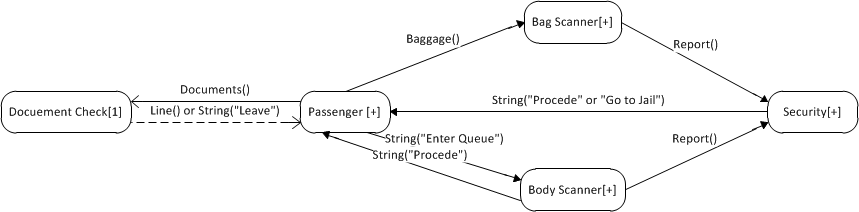
\includegraphics[width=\textwidth]{actorCollabDiagram.png}
\caption{Actor collaboration diagram}
\end{figure}

\end{document}
